\chapter{Möglichkeiten der ISO 29002-31 - Exchange of characteristics data}

Die ISO 29002-31 ermöglicht abstrakt folgende Arten von Abfragen:
\begin{itemize}
\item Liefern oder validieren der spezifizierten characteristic data für das mittels Identifier angegebene Element.
\item Liefern des Identifiers eines Elementes welches den übermittelten characteristic data (am ehesten) entspricht. 
\end{itemize}

\section{XML Datencontaineranalyse}
Die Unterkapitel beschreiben die einzelnen (XML) Datencontainer aus der ISO 29002-31. Der Ausgangspunkt ist der query\_context, welcher einige Metadaten zum eigentlichen query enthält. 

\subsection{query\_context}
Dies ist eine Art Container für eine Menge von Queries. Inhalt sind Informationen über den Anforderer der Daten zwecks persönlicher Kontaktaufnahme, wie z.B. die Anfragezeit, Informationen über die Organisation welche die Anfrage schickt sowie einen gewünschten Antwortzeitpunkt mit Antwort-Email Adresse. 


\subsection{query}
Die Unterstützung aller Funktionalitäten des queries entspricht laut ISO 29002-31 Anhang 6 der Conformance class 1: simple query.
Dies ist der eigentliche Abfrage-Datensatz. Abgefragt werden kann mittels class IRDI, data\_specification IRDI\footnote{IRDI  - International registration data identifier}, eine Menge von property IRDI, Item Daten (das sind Items gefüllt mit Daten die bereits bekannt sind) und einer item\_description. Das bedeutet, dass bereits bekannt Properties eines Items übertragen werden können, um die Suche zu vereinfachen.

Der query beihaltet folglich auch die data\_specification IRDI. Diese verweist auf eine Spezifikation aus ISO 22754-30, die besagt welche Properties für dieses Item sinnvoll sind. Die angegebenen Property IRDIs sind dann eine Teilmenge aus den mittles data\_specification IRDI definierten erlaubten properties. 

Ad hoc denkbar wären einfache Abfragens wie z.B.: "Gib mir alle Items der Klasse xyz". Mitgeliefert werden auch Items von Subklassen. Weiterhin kann die Abfrage nach bestimmten Properties eingeschränkt werden. Eine weitere Möglichkeit ist es bereits bekannte Daten über ein Element zu übermitteln, mit dem Zwecke hierüber die IRDI zu erfahren oder weitere Property-Daten zu erhalten. Siehe Beispielqueries simple queries in Kapitel \ref{kap:query_beispiele}. 

\subsection{characteristic\_data\_query\_expression (parametric\_query)}
Das entspricht laut ISO 29002-31 Anhang 6 der Conformance class 2: parametric query.

Eine characteristic\_data\_query\_expression kann verschieden expressions vom Typ query\_expression beinhalten. Von jedem Typ jeweils nur maximal eine. 
Z.B.
\begin{itemize}
\item string\_size\_expression
\item string\_pattern\_expression
\item range\_expression
\item data\_environment\_expression
\item cardinality\_expression
\item subset\_expression
\end{itemize}
darüberhinaus noch folgende Attribute

\begin{itemize}
\item property\_reference - die property auf den die query\_expression bezogen ist
\end{itemize}
Solch eine Expression ermöglicht das Filtern, gleichsam ein Einschränken bestimmter Properties und Werte. 

\subsection{Query Beispiele}\label{kap:query_beispiele}

Eine Schraube hat die folgenden möglichen Properties: 

\begin{description}
\item[Klassen-Identifier] 1234-abcd\# ab-cdefgh\# 1 (IRDI)
\item[Typ] M6 (Property IRDI: 1234-abcd\# ab-bbbbbb\# 1)
\item[Länge] 80mm (Property IRDI: 1234-abcd\# ab-cccccc\# 1)
\end{description}

\subsubsection{Simple Query}

Jetzt ermöglicht ein simpler query folgende Abfrage: "Gib mir alle Items zu der Klasse Kreuzschraube mit dem Identifier (IRDI) 1234-abcd\# ab-cdefgh\# 1. Das Ergebnis ist ein Item, mit allen Attributen wie oben angegeben. 

Ein anderer Query könnte lauten: "Gib mir die Properties 1234-abcd\# ab-cccccc\# 1 und 1234-abcd\# bbbbbb\# 1 des Items der Klasse 1234-abcd\# ab-cdefgh\# 1". Das Ergebnis wäre das Item mit Typ: M6 und die Länge: 80mm.

Es könnte auch mit Hilfe von vorhandenen Daten gesucht werden, z.B.: "Hier ist ein Item mit der Property Typ: M6 (Property IRDI: 1234-abcd\# ab-bbbbbb\# 1), gibt mir bitte dazu die Properties 1234-abcd\# ab-cccccc\# 1 und 1234-abcd\# bbbbbb\# 1 

\subsubsection{Parametric Query}

Hat man jetzt noch eine Schraube mit folgenden Eigenschaften:
\begin{description}
\item[Klassen-Identifier] 1234-abcd\# ab-cdefgh\# 1 (IRDI)
\item[Typ] M5 (Property IRDI: 1234-abcd\# xx-bbbbbb\# 1)
\item[Länge] 100mm (Property IRDI: 1234-abcd\# xx-cccccc\# 1)
\end{description}


Mit Hilfe der characteristic\_data\_query\_expression sind folgende Abfragen möglich: "Gib mir die Properties 1234-abcd\# ab-cccccc\# 1 (Länge) und 1234-abcd\# bbbbbb\# 1 (Typ) der Klasse Klasse 1234-abcd\# ab-cdefgh\# 1 (Schraube) wo die Länge zwischen 50 und 150mm und der Typ M5 oder M6 sein soll."


Diese ermöglicht das filtern auf genau eine übergebene Property. Rekursive Abfragen sind auch möglich, beispielsweise wenn die gesuchte Property eine Multi-Property ist (Property: Loch als Wert zwei Properties mit Form und Durchmesser und Durchmesser soll gefiltert werden)

\section{Was ermöglicht die ISO 22745-30}

Ein Identification Guide beschreibt welche Daten für ein Objekt benötigt werden, damit dies überhaupt sinnvoll für einen bestimmten Zweck eingesetzt werden kann. Der Käufer, Produktmanager oder Benutzer definiert die Anforderungen an die Daten. Ein "Datenanforderungsstatement" wird als ein eOTD-i-xml identification guide xml file erzeugt. Es wird definiert, was der Name des Artikels ist mit den charakteristischen Daten. Es wird die Frage beantwortet, welche Daten (Properties) zu einer bestimmten Klasse eines Objektes benötigt wird um den Artikeln zu kaufen oder zu sinnvoll zu verwalten. Diese Anforderungen werden von der Abfrageseite (Kundenseite) definiert, also derjenige, der Daten abfragen möchte. \(Quelle: ECCMA\_ISO\_8000\_certification.pdf\)
Ein Identification guide referenziert Konzepte eines Dictionaries um Datenanforderungen einer bestimmten Klasse zu beschreiben. (ISO 22745-30 Kapitel 5). 
Ein Datenempfänger kann eine Organisation oder eine Gruppe von Organisationen oder Firmen sein, welche ähnliche Datenanforderungen haben. Somit wird ein Identification Guide Gruppe von einer speziellen Organisation verwaltet, welche wiederum selbst Datenempfänger sein kann.  

\section{Offene Fragen}

\subsection{ISO 29002-31}
\begin{description}
\item[Abfrage Schnittstelle] Der Standard gibt keine genaue Implementierung vor, erwähnt aber eine Anfrage per E-Mail. Hierfür vermutlich auch die Antwortadresse zwecks automatisierter Antwort ebenfalls per Mail. Wir haben uns bereits auf Web Service geeinigt, da es naheliegt. Kapitel 6 besagt, dass der query\_context entfallen kann falls ein anderer "Hüllen"-Standard wie z.B. EDI genutzt wird. Ich denke das trifft hier zu. 
\item[Conformance class] Welche conformance class sollen wir unterstützen? CC1 - simple query, oder CC2 - parametric query?
\item[XSD] Im Anhand sind XSDs referenziert. Diese wären natürlich für die Implementierung hilfreich.
\item[data\_specification reference] Es wird eine data\_specification\_reference als IRDI mit dem query übermittelt. Womit wird das abgeglichen? Siehe dazu auch weiter unten, die Fragen zu ISO 22745-30.
ISO 29002-31 sagt: 
\begin{quotation}
A query can reference a data specification, which defines the properties for the class of items being queried. The format of the data specification is not specified in this part of ISO/TS 29002. ISO 13584-32 or ISO/TS 22745-30 specify data models and exchange formats that could be used for data specifications.
\end{quotation}
\end{description}


\subsection{ISO 22745-30}
\begin{description}
\item[IG Anwendung] Da der Identification Guide beschreibt, welche Daten überhaupt sinnvoll sind, stellt sich die Frage wohin diese Abfrage gestellt wird. Verstanden habe ich es so, dass der Kunde jeweils selbst diese Daten pflegt. Die ISO 22745-30 sagt dazu \begin{quote}
Most data recipients require data describing items belonging to more than one class. An identification guide group is a collection of identification guides that, together, describe the data recipient's requirements for describing items belonging to more than one class.
\end{quote} Es ist offensichtlich so, dass der Datenempfänger definiert welche Datenqualität er benötigt und welche nicht. 
Folglich verstehe ich das so, dass der IG nicht gleichzusetzen mit einem "select" in SQL ist, sondern beschreibt welche Properties einer Class abgefragt werden sollten damit überhaupt sinnvoll damit umgegangen werden kann, denn das Dictionary wird offensichtlich eine große Menge an Properties beinhalten die für bestimmte Kunden für dessen Anwendung nicht sinnvoll sind. Stellt sich die Frage, ob ich den IG umsetzen soll? Der "select"-Teil eines Queries kann bereits mit 29002-31 gestellt werden, nur weiß der Kunde nicht welche Properties er für einen bestimmten selbstdefinierten Zweck benötigt. Das muss er vorab definieren. Aber ein XML aus 22745-30 welche das beschreibt wird nicht an den Datenbereitsteller geschickt. 
EIn Identification Guide wird auch verglichen mit einem Formular, welches definiert welche Formularfelder enthalten sein sollen. Man könnte somit das Abfrageformular hieraus generieren. Stellt sich die Frage ob dies so dynamisch sinnvoll ist. 
\item[IG Abfrage] Soll der IG umgesetzt werden, ist mir nicht klar, wie das passieren soll. Beschrieben wird in diversen Präsentationen aus dem Internet \(z.B. ECCMA^\_ISO\_8000\_certification.pdf\), dass der IG sich auf Kundenseite befindet. 
Wie erfolgt die Abfrage dann? Auf welcher Datenbasis? Wohin wird solch eine Abfrage geschickt bzw woher wird die Spezifikation der Datenqualität geholt? Siehe Abbildung \ref{fig:ig_query_response}

\item[XSD] Im Anhand sind XSDs referenziert. Diese wären natürlich für die Implementierung hilfreich.
\end{description}


\begin{figure}[htbp]
	\centering
		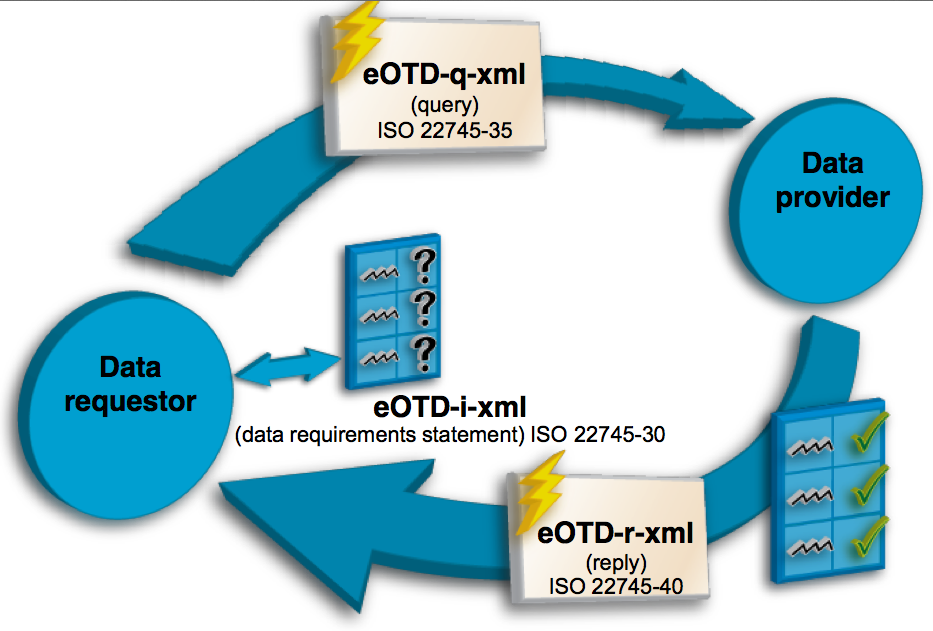
\includegraphics[width=0.8\textwidth]{images/ig_query_response.png}
	\caption{Ablauf eines queries}
	\label{fig:ig_query_response}
\end{figure}
